%%%%%%%%%%%%%%%%%%%%%%%%%%%%%%%%%%%%%%%%%%%%%%%%%%%%%%%%%%%%%%%%%%%%%%%%%%%%%%%%
%2345678901234567890123456789012345678901234567890123456789012345678901234567890
%        1         2         3         4         5         6         7         8

\documentclass[letterpaper, 10 pt, conference]{ieeeconf}  % Comment this line out if you need a4paper

%\documentclass[a4paper, 10pt, conference]{ieeeconf}      % Use this line for a4 paper

\IEEEoverridecommandlockouts                              % This command is only needed if 
                                                          % you want to use the \thanks command

\overrideIEEEmargins                                      % Needed to meet printer requirements.

% See the \addtolength command later in the file to balance the column lengths
% on the last page of the document

% The following packages can be found on http:\\www.ctan.org
%\usepackage{graphics} % for pdf, bitmapped graphics files
%\usepackage{epsfig} % for postscript graphics files
%\usepackage{mathptmx} % assumes new font selection scheme installed
%\usepackage{times} % assumes new font selection scheme installed
\usepackage{float}
\usepackage{ngerman}
\usepackage[utf8]{inputenc}
\usepackage{color}
\usepackage{amsmath}
\usepackage{bm}
\usepackage{amssymb}
\usepackage{graphicx}
\graphicspath{{./figures/}}
% Symbole für Tabelle: grüner Haken und rotes Kreuz
\newcommand{\ok}{{\color{green}\checkmark}}
\newcommand{\no}{{\color{red}$\boldsymbol\times$}}


\title{\LARGE \bf
Kinematics and Dynamics Model of an Exoskeleton for Craftsmen Force Assistance via explicit Elimination of Kinematic Constraints
}


\author{Moritz Schappler$^{1}$ and Sami Haddadin$^{2}$% <-this % stops a space
\thanks{*This work was supported by the German Federal Ministry of Education and Research under Grant no. 16SV6175}% <-this % stops a space
\thanks{$^{1}$Moritz Schappler
        {\tt\small schappler@irt.uni-hannover.de}}%
\thanks{$^{2}$Sami Haddadin
        {\tt\small haddadin@irt.uni-hannover.de}}%
}


\begin{document}



\maketitle
\thispagestyle{empty}
\pagestyle{empty}


%%%%%%%%%%%%%%%%%%%%%%%%%%%%%%%%%%%%%%%%%%%%%%%%%%%%%%%%%%%%%%%%%%%%%%%%%%%%%%%%
\begin{abstract}

abstract

\end{abstract}


%%%%%%%%%%%%%%%%%%%%%%%%%%%%%%%%%%%%%%%%%%%%%%%%%%%%%%%%%%%%%%%%%%%%%%%%%%%%%%%%
\section{Introduction and State of the Art}

Exoskeletons for assistance and rehabilitation

list different upper limb exoskeletons with different concepts


\section{Exoskeleton and Scenario}

\subsection{Scenario}

force assistance for craftsmen
project goals \cite{NuelleSchTapLil2017}: 
* reduce fatigue of the worker and work-induced diseases, 
* increase work quality by projection of additional information (augmented reality, \cite{NuelleBriTapDem2018})
* guiding the user

\subsection{Exoskeleton}

building upon \cite{PetereitAlbJerSch2012}

presentation of two demonstrators in the project
KAS4, KAS5
components: Short review of the single components

\subsubsection{main structure next to the human arm}

\begin{figure}[tb!]
    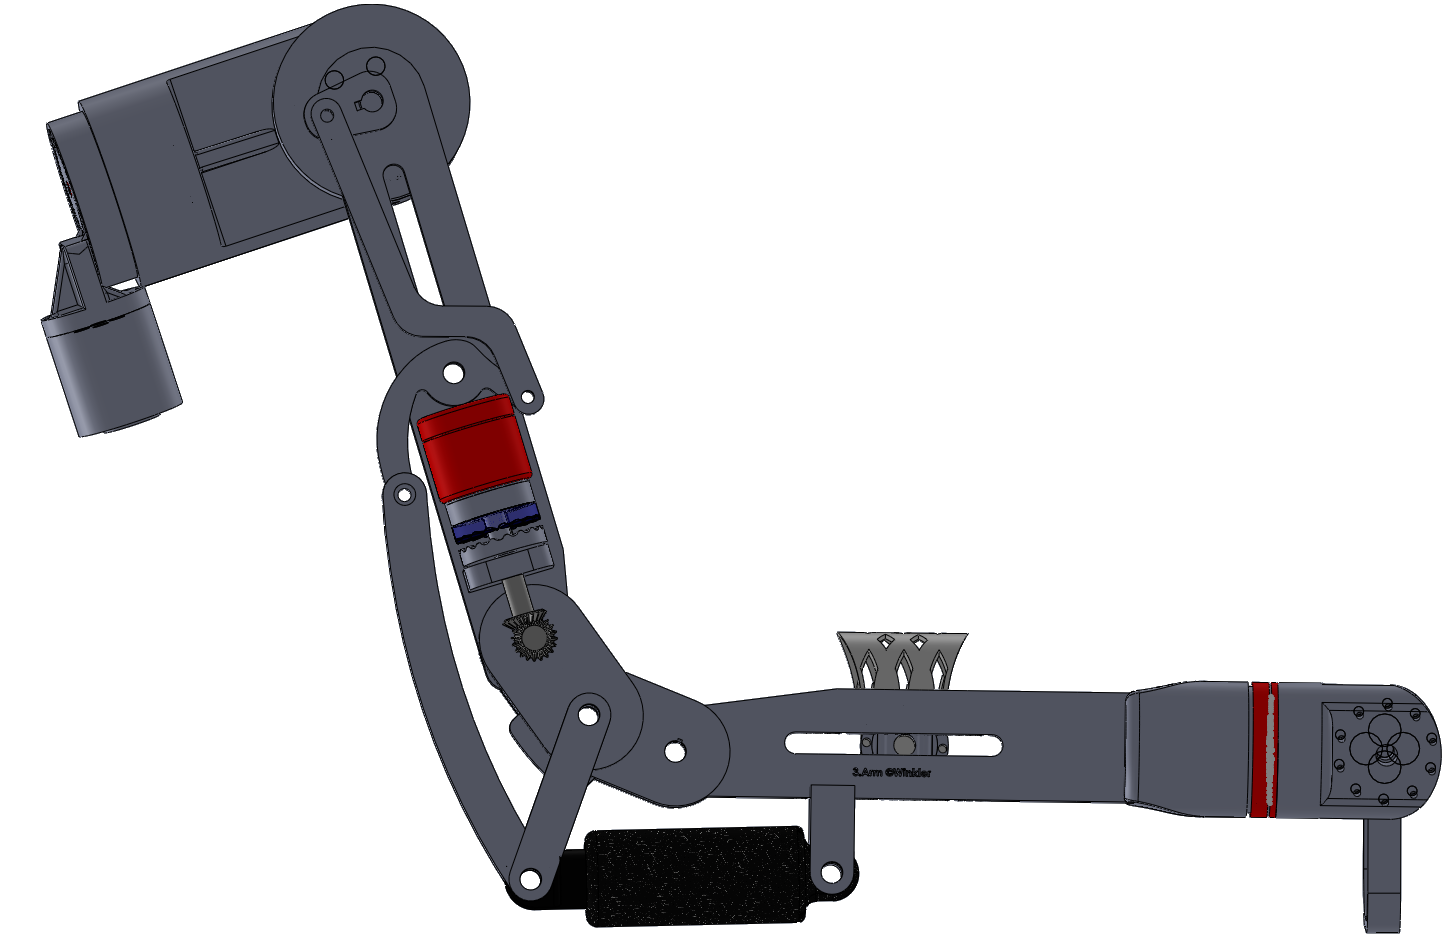
\includegraphics[width=\linewidth]{figures/KAS5_Seitenansicht_CAD_Ausschnitt_transp.png}
    \caption{CAD-Modell KAS5}
    \label{fig:KAS5_CAD}
\end{figure} 

\subsubsection{three-axis-elbow joint}


\begin{figure}[tb!]
    \begin{tabular}{c c c}
        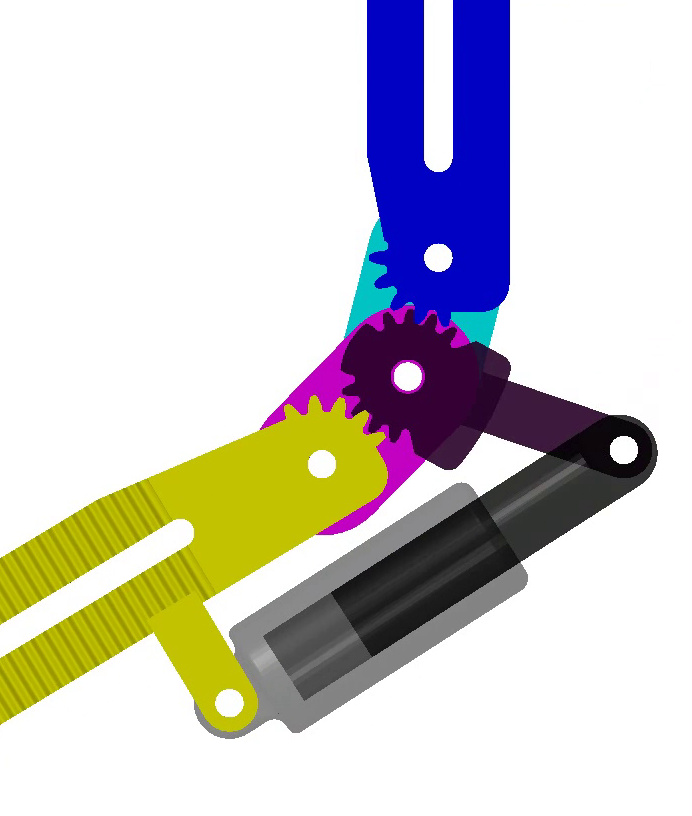
\includegraphics[width=0.28\linewidth]{figures/KAS6m3_SimMech_1.png} &
        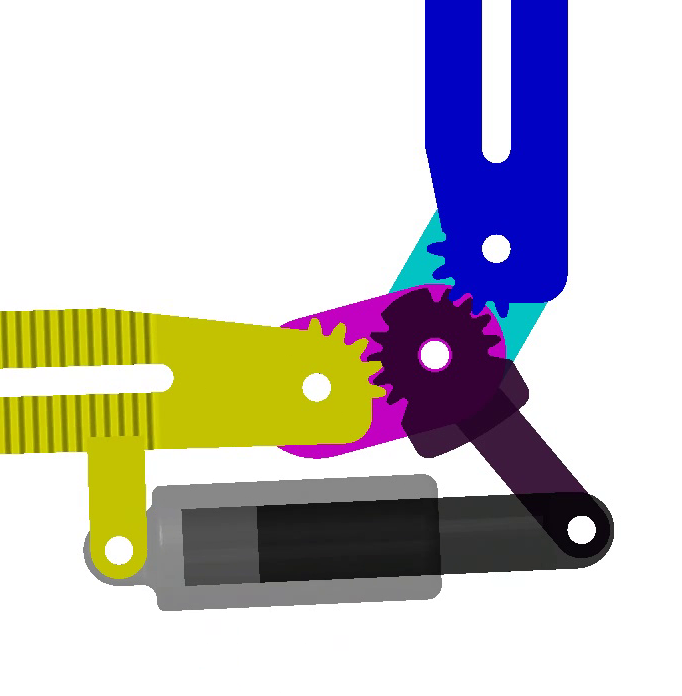
\includegraphics[width=0.30\linewidth]{figures/KAS6m3_SimMech_2.png} &
        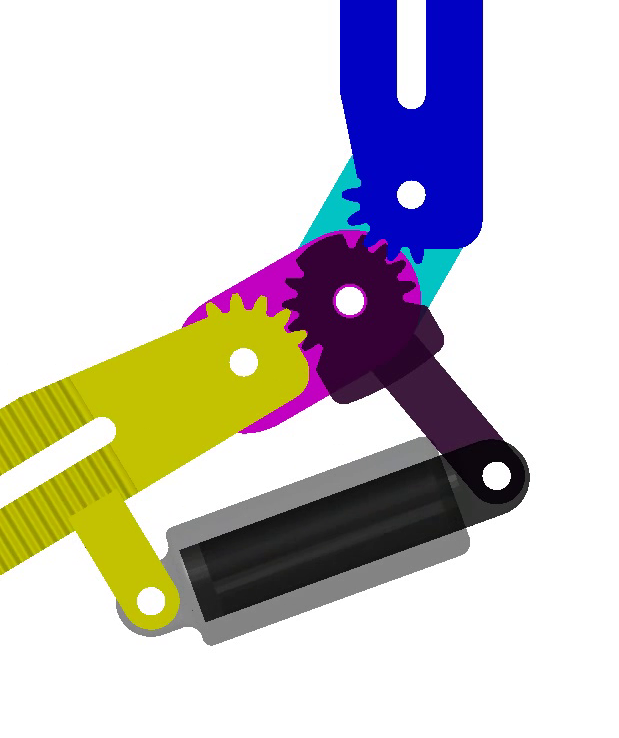
\includegraphics[width=0.28\linewidth]{figures/KAS6m3_SimMech_3.png}
    \end{tabular}

    \caption[Überprüfung der Kinematik in SimMechanics]{Überprüfung der Kinematik in SimMechanics am Beispiel unterschiedlicher Stellungen des KAS6. Damit lässt sich visuell ein korrektes Abrollen der Verzahnungen prüfen.}
    \label{fig:EllenbogenSimMech}
\end{figure} 

\subsubsection{three-axis shoulder joint}

\subsubsection{lever-mechanism for force transmission to the elbow joint}

\subsubsection{lever-mechanism for force transmission from the shoulder to the elbow}

\subsubsection{mechanical spring-damper system}

\section{Kinematics and Dynamics Modelling}

\subsection{Kinematic Model}

\begin{tabular}[t]{|c||c|c|c|c|c|}
    \hline
    $i$ & $\alpha_i$ & $d_i$ & $\theta_i$ & $r_i$ & $a(i)$ \\
    \hline
    1 & $0$ & $0$ & $\rho_1-\pi/2$ & $l_1$ & 0 \\
    2 & $-\pi/2$ & $0$ & $\rho_2+\pi/2$ & $l_2$ & 1 \\
    3 & $\pi/2$ & $0$ & $\rho_3$ & $l_3$ & 2 \\
    4 & $0$ & $l_5$ & $\rho_4$ & $0$ & 3 \\
    5 & $0$ & $l_{11}$ & $\rho_5$ & $0$ & 4 \\
    6 & $0$ & $l_{12}$ & $\rho_6$ & $0$ & 5 \\
    7 & $\pi/2$ & $0$ & $\rho_7$ & $l_{15}$ & 6 \\
    8 & $\pi/2$ & $0$ & $\delta_{1}+\pi/2$ & $l_{3}$ & 2 \\
    9 & $0$ & $-l_{4}$ & $-\delta_{2}$ & $0$ & 8 \\
    10 & $0$ & $l_{6}$ & $-\delta_{3}$ & $0$ & 3 \\
    11 & $0$ & $l_{22}$ & $\pi-\delta_{4}$ & $0$ & 10 \\
    12 & $0$ & $l_{11}$ & $\delta_{5}-\pi/2$ & $0$ & 4 \\
    13 & $0$ & $l_{11}$ & $\delta_{6}-\pi/2$ & $0$ & 12 \\
    14 & $0$ & $0$ & $3\pi/2-\delta_{7}$ & $0$ & 13 \\
    15 & $\pi/2$ & $0$ & $0$ & $l_{\mathrm{F}}$ & 14 \\
    \hline
\end{tabular}

\begin{figure}[htb]
    \tiny
    \begin{minipage}[t]{7.5cm}
        \vspace{0.2cm} % wird für bounding box des Bilds benötigt
        \input{./figures/KAS5_m3_skizze_kinematik_2_KS.pdf_tex}
    \end{minipage}

    \caption[Kinematikmodell und Skizze des KAS5]{Kinematikmodell und Skizze des KAS5 nach \cite{KhalilKle1986}. Starrkörper sind durch entsprechende eingekreiste Nummern (entspricht Tabellenspalte \glqq{}$i$\grqq{}) und körperfeste Koordinatensysteme gekennzeichnet. Die Körper 8, 9, 10, 11, 13 sind die Kurbeln und Hebel der Parallelstruktur}
    \label{fig:KAS5_kinematik}
\end{figure}

Joint coordinates $\bm{q}$ of the unconstrained system can according to \cite{NakamuraGho1989} be separated into the  minimal coordinates
%
\begin{equation}
\bm{q}_1=\begin{pmatrix}\rho_1 & \rho_2 & \rho_4 & \rho_5 &\rho_7 \end{pmatrix}^\mathrm{T}
\end{equation}
%
and the dependant coordinates
%
\begin{equation}
\bm{q}_2=\begin{pmatrix}\rho_3 & \delta_1 & ... \end{pmatrix}^\mathrm{T}.
\end{equation}

\subsection{Eliminiation of Kinematic Constraints}


\subsubsection{elbow joint}

describe gear constraints.

Velocity calculation of the pitch points.

Das Abwälzen der Zahnräder im Ellenbogen wird über eine Gleichung der Ellenbogenwinkel $\rho_4,\rho_5,\rho_6$ modelliert.

corresponds to additional constraints, not generated by closed loops

\subsubsection{elbow-shoulder-coupling}

define circles: geometrical method to solve the kinematic constraints for the closed loops
calculate intersection points of the two circles via quadratic equations 

iterative procedure (first circle, second circle)

\subsubsection{complete model}



Es muss nicht die explizite Lösung der Zwangsbedingungen aus (\ref{equ:ZB_explizit}) gefunden werden, sondern nur die explizite Form für 
%
\begin{align}
\mathrm{sin}(\bm{q}_2) =& \bm{f}_\mathrm{sin}(\bm{q}_1) \\
\mathrm{cos}(\bm{q}_2) =& \bm{f}_\mathrm{cos}(\bm{q}_1) \\
\dot{\bm{q}}_2 =& \bm{f}_\mathrm{diff}(\bm{q}_1,\dot{\bm{q}}_1).
\end{align}


\subsection{Dynamics Model}

\label{sec:Lagrange2Elim}
%
Diese Form wird in den Energiegleichungen benötigt.
Vor der Elimination der ZB ist das Lagrange-Funktional $L$ in der Form
\begin{equation}
L(\bm{q},\dot{\bm{q}})=L(\mathrm{sin}(\bm{q}_1),\mathrm{cos}(\bm{q}_1),\dot{\bm{q}}_1,\mathrm{sin}(\bm{q}_2),\mathrm{cos}(\bm{q}_2),\dot{\bm{q}}_2).
\end{equation}
Nach der Substitution sind sie in der für Lagrange 2. Art geeigneten Form in Darstellung der Minimalkoordinaten $\bm{q}_1$
%
\begin{equation}
L(\bm{q}_1,\dot{\bm{q}}_1)=L(\mathrm{sin}(\bm{q}_1),\mathrm{cos}(\bm{q}_1),\dot{\bm{q}}_1,\bm{f}_\mathrm{sin}(\bm{q}_1),\bm{f}_\mathrm{cos}(\bm{q}_1), \bm{f}_\mathrm{diff}(\bm{q}_1,\dot{\bm{q}}_1)).
\end{equation}
%
Mit dem Lagrange-Formalismus
%
\begin{equation}
\frac{\mathrm{d}}{\mathrm{d}t}\frac{\partial L(\bm{q}_1,\dot{\bm{q}}_1)}{\partial \dot{\bm{q}}_1} - \frac{\partial L(\bm{q}_1,\dot{\bm{q}}_1)}{\partial \bm{q}_1} = \bm{\tau}^c_1,
\end{equation}
%
der auch in \cite{NakamuraGho1989} zur Herleitung von (\ref{equ:tau_Projektion}) benutzt wurde, folgt wieder die gesuchte Dynamik-Darstellung aus (\ref{equ:Dyn_MinKoord}).

%
%Für Newton-Euler bräuchte man noch $d^2(x)/dt^2=...$.
%Diese Formen sind effizienter zu berechnen als die explizite Form $x=...$ (auf die dann wieder $sin()$, $cos()$ angewendet würde).
Das wurde in \cite{WangGosselin1998} schon so gemacht. Dort aber nicht wirklich hervorgehoben.

\section{Control Concept}

joint torque based gravity compensation

\section{Simulation Environment}

forward dynamics
simulink model
human user as force/torque in free space for first evaluations
coupling with musculo-skeletal model \cite{KuehnHuSchHad2018}


\section{Simulation Results}

energy consistency

\begin{figure*}[tb!]
    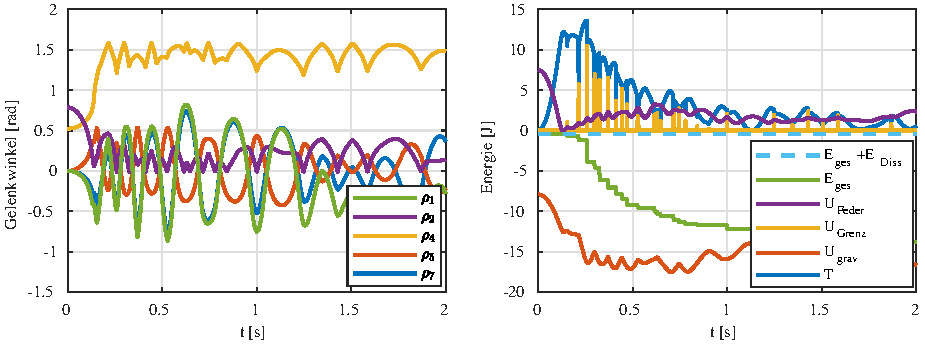
\includegraphics{figures/KAS5m5_Gelenkgrenzmodell_q_E.pdf} 
    \caption[Zeitverläufe aus der Simulation zur Prüfung der Energiekonsistenz]{Zeitverläufe aus der Simulation zur Prüfung der Energiekonsistenz. Links: Gelenkwinkel. Rechts: Energien (kinetische Energie $T$, Gravitationspotential $U_\mathrm{grav}$, Federenergie der modellierten Gelenkwinkelanschläge $U_\mathrm{Grenz}$, Federenergie der Linearfeder $U_\mathrm{Feder}$, Gesamtenergie $E_\mathrm{ges}$, Dissipierte Energie $E_\mathrm{Diss}$)}
    \label{fig:SimulationEnergiekonsistenz}
\end{figure*} 


improving gravity compensation

\section{Conclusions}

A conclusion.

\addtolength{\textheight}{-12cm}   % This command serves to balance the column lengths
                                  % on the last page of the document manually. It shortens
                                  % the textheight of the last page by a suitable amount.
                                  % This command does not take effect until the next page
                                  % so it should come on the page before the last. Make
                                  % sure that you do not shorten the textheight too much.

%%%%%%%%%%%%%%%%%%%%%%%%%%%%%%%%%%%%%%%%%%%%%%%%%%%%%%%%%%%%%%%%%%%%%%%%%%%%%%%%



%%%%%%%%%%%%%%%%%%%%%%%%%%%%%%%%%%%%%%%%%%%%%%%%%%%%%%%%%%%%%%%%%%%%%%%%%%%%%%%%



%%%%%%%%%%%%%%%%%%%%%%%%%%%%%%%%%%%%%%%%%%%%%%%%%%%%%%%%%%%%%%%%%%%%%%%%%%%%%%%%
%\section*{APPENDIX}
%
%Appendixes should appear before the acknowledgment.


\section*{ACKNOWLEDGMENT}

...


%%%%%%%%%%%%%%%%%%%%%%%%%%%%%%%%%%%%%%%%%%%%%%%%%%%%%%%%%%%%%%%%%%%%%%%%%%%%%%%%


% BIBLIOGRAPHY
\bibliographystyle{ieeetr}
\bibliography{ref}
\end{document}
